\documentclass[11pt,a4paper]{article}
\usepackage{gtu-el-yazisi}
\begin{document}
\notbilgi{Analog Haberleşme}{Lineer sistemlerde işaret iletimi; enerji ve güç spektral yoğunluğu}{Ders5.pdf}

\section{Lineer sistemlerden işaretlerin iletilmesi}
\sayfa{1}
\begin{center}
\begin{tikzpicture}[>=Stealth, line width=0.7pt]
  \node[draw, minimum width=1.6cm, minimum height=0.9cm] (h) at (0,0) {$h(t)$};
  \draw[->] (-2.4,0) -- (h.west);
  \node[below] at (-1.9,0) {$x(t)$};
  \draw[->] (h.east) -- (1.8,0);
  \node[right] at (1.8,0) {$y(t)=x(t)\ast h(t)$};
  \node[font=\small] (dc) at (1.6,1.1) {Dürtü cevabı};
  \draw[->] (dc.west) to[bend right] (h.north east);
\end{tikzpicture}
\end{center}
\begin{align*}
  & Y(f) = X(f)\cdot H(f) \qquad (H(f):\ \text{Transfer fonk.}) \\
  & |Y(f)|\,e^{j\theta_y(f)} = |X(f)|\,e^{j\theta_x(f)}\cdot|H(f)|\,e^{j\theta_h(f)} \\
  & |Y(f)| = |X(f)|\cdot|H(f)| \\
  & \theta_y(f) = \theta_x(f)+\theta_h(f)
\end{align*}

\begin{ornek}
  \begin{center}
  \begin{tikzpicture}[>=Stealth, line width=0.7pt]
    \node[draw, line width=1.1pt, minimum width=1.2cm, minimum height=0.8cm] (h) at (0,0) {$h(t)$};
    \draw[->] (-2.0,0) node[left] {$x(t)$} -- (h.west);
    \draw[->] (h.east) -- (2.0,0) node[right] {$y(t)$};
  \end{tikzpicture}
  \end{center}
  $x(t)=3+5\cos\!\left(3t+\dfrac{\pi}{4}\right)$, \qquad
  $H(f)=j20\pi f = 10\cdot j2\pi f \;\Rightarrow\; h(t)=10\,\dfrac{d}{dt}(\ )$

  a) $x(t)$'nin periyodu? $y(t)$'nin periyodu? \quad
  b) $P_x=\,$? \quad c) $y(t)=\,$? \quad d) $P_y=\,$?
\end{ornek}

a) $x(t)=3+5\cos\!\big(\underbrace{3}_{\omega_0}t+\tfrac{\pi}{4}\big)$ \qquad
$\omega_0=3=2\pi f_0=\dfrac{2\pi}{T_0} \;\rightarrow\; T_{0x}=\dfrac{2\pi}{3}$

\textcolor{kirmizikalem}{$\star$ LTI sistemde çıkışın frekansı giriş ile aynıdır}

LTI $\Rightarrow\; T_{0,y}=T_{0,x}=\dfrac{2\pi}{3}$

b) $P_x = 3^2+\dfrac{5^2}{2} = 21{,}5$ watt \qquad ($\omega_0=3=2\pi f_0 \;\Rightarrow\; f_0=\dfrac{3}{2\pi}$)
\[
  x(t)=\underbrace{3}_{x_0}+\underbrace{\frac{5}{2}e^{j\pi/4}}_{x_1}\,e^{j\underset{\omega_0}{3}t}
  +\underbrace{\frac{5}{2}e^{-j\pi/4}}_{x_2}\,e^{-j\overset{\omega_0}{3}t}
\]
\[
  \rightarrow\; P_x=\sum_n |x_n|^2 = 3^2+\left(\frac{5}{2}\right)^2+\left(\frac{5}{2}\right)^2 = 21{,}5\ \text{watt}
\]

c) $Y(f)=X(f)\cdot H(f)$
\begin{align*}
  H(f) &= j20\pi f \\
  X(f) &= 3\delta(f)+\frac{5}{2}e^{j\pi/4}\,\delta(f-f_0)+\frac{5}{2}\,e^{-j\pi/4}\,\delta(f+f_0) \\
  Y(f) &= H(f)\cdot X(f) = (j20\pi f)\left[3\delta(f)+\frac{5}{2}e^{j\pi/4}\delta(f-f_0)+\frac{5}{2}e^{-j\pi/4}\delta(f+f_0)\right] \\
  &= \underbrace{3\delta(f)\cdot j20\pi(0)}_{0} + j20\pi\left(\frac{3}{2\pi}\right)\cdot\frac{5}{2}\,e^{j\pi/4}\,\delta(f-f_0) \\
  &\quad + j20\pi\left(-\frac{3}{2\pi}\right)\frac{5}{2}\,e^{-j\pi/4}\,\delta(f+f_0)
\end{align*}

\sayfa{2}
\begin{align*}
  &= 75\,\underbrace{j\,e^{j\pi/4}}_{e^{j3\pi/4}}\,\delta(f-f_0)\;\textcolor{kirmizikalem}{-}\;75\,\underbrace{j\,e^{-j\pi/4}}_{\textcolor{kirmizikalem}{e^{-j3\pi/4}}}\,\delta(f+f_0) \\
  Y(f) &= 75e^{j3\pi/4}\,\delta(f-f_0)+75e^{-j3\pi/4}\,\delta(f+f_0)
\end{align*}
$\mathcal{F}^{-1}\ \downarrow$
\begin{align*}
  y(t) &= 150\cos\!\Big(\overbrace{2\pi f_0}^{3}\,t+\frac{3\pi}{4}\Big) \\
  P_y &= \frac{150^2}{2}\ \text{watt} = 11250
\end{align*}

\begin{center}
\begin{tikzpicture}[>=Stealth, line width=0.8pt]
  \node[draw, minimum width=2.6cm, minimum height=1.6cm] (h) at (0,0) {$h(t)$};
  \draw[->] (-3.8,0) -- (h.west);
  \node[below, align=center, font=\small] at (-3.0,0) {$x(t)$\\ periyodik};
  \draw[->] (h.east) -- (3.8,0);
  \node[below, align=center, font=\small] at (3.0,0) {$y(t)$\\ periyodik};
\end{tikzpicture}
\end{center}
\begin{align*}
  x(t) &= \sum_n x_n\,e^{j2\pi n f_0 t} & y(t) &= \sum_n y_n\,e^{j2\pi n f_0 t} \\
  X(f) &= \sum_n x_n\,\delta(f-nf_0) & Y(f) &= \sum_n y_n\,\delta(f-nf_0)
\end{align*}
\begin{align*}
  Y(f) &= H(f)X(f) = H(f)\sum_n x_n\,\delta(f-nf_0) \\
  &= \sum_n x_n\,\underbrace{H(f)\,\delta(f-nf_0)}_{H(nf_0)\cdot\delta(f-nf_0)}
\end{align*}
\[
  \kutula{Y(f)=\sum_n \underbrace{x_n H(nf_0)}_{y_n}\,\delta(f-nf_0)}
  \;\xrightarrow{\ \mathcal{F}^{-1}\ }\; y(t)=\sum_n y_n\,e^{j2\pi n f_0 t}
\]

\textcolor{kirmizikalem}{\okunamadi{Önch} ex 2.2.6 inceleyiniz (57--59, 1. baskı)}

\section{Enerji ve Enerji yoğunluk fonksiyonu (EYF)}
\subsection{Energy Spectral Density (ESD)}
\begin{align*}
  E_x &= \int_{-\infty}^{\infty}|x(t)|^2\,dt = \int_{-\infty}^{\infty}x(t)\cdot x^*(t)\,dt = \\
  &= \int_{-\infty}^{\infty}x(t)\Bigg[\underbrace{\int_{-\infty}^{+\infty}X(f)\,e^{j2\pi f t}\,df}_{=\int_{-\infty}^{\infty}X^*(f)\,e^{-j2\pi f t}}\Bigg]^{*}dt
\end{align*}

\sayfa{3}
\begin{align*}
  &= \int_{-\infty}^{\infty}X^*(f)\,\underbrace{\int_{-\infty}^{\infty}x(t)\,e^{-j2\pi f t}\,dt}_{X(f)}\,df \\
  &= \int_{-\infty}^{\infty}|X(f)|^2\,df
\end{align*}
\textcolor{kirmizikalem}{Parseval t.:}
\[
  E_x=\int_{-\infty}^{\infty}|x(t)|^2\,dt=\int_{-\infty}^{\infty}\underbrace{|X(f)|^2}_{\mathcal{E}_x(f):\ \text{EYF}}\,df
\]
\begin{center}Enerji Tayf yoğunluğu F(EYF)\end{center}

\subsection{Enerji işaretleri için özilişki fonk (autocorrelation)}
\begin{align*}
  \underbrace{R_x(\tau)}_{x(t)\text{'nin özilişki fonk}} &= \int_{-\infty}^{+\infty}x(t)\cdot x^*(t-\tau)\,dt = \int_{-\infty}^{\infty}x(t)\,x^*(t+\tau)\,dt \\
  &= \int_{-\infty}^{+\infty}x^*(t)\,x(t+\tau)\,dt
\end{align*}
\begin{align*}
  R_x(-\tau) &= R_x(\tau) \quad \text{çift fonksiyondur} \\
  R_x(\tau) &= x(\tau)\ast x(-\tau)
\end{align*}
$x(t)$ reel olsun $\Rightarrow\ R_x(\tau)=x(\tau)\ast x(-\tau)$

\hspace{4cm}$\downarrow\mathcal{F}$
\begin{align*}
  \mathcal{F}\{R_x(\tau)\} &= X(f)\cdot\frac{1}{|-1|}\,X\!\left(\frac{f}{-1}\right) \\
  &= X(f)\cdot\underbrace{X(-f)}_{X^*(f)}
\end{align*}
$x(t)$ reelse $X(f)=X^*(-f)$
\[
  \mathcal{F}^{-1}\{R_x(\tau)\}=|X(f)|^2=\mathcal{E}_x(f)\footnotemark
\]
\footnotetext{Claude notu: $\mathcal{F}$ üzerindeki işaret okunaksız; formüle göre $\mathcal{F}\{R_x(\tau)\}$ olmalı.}
\formulkutu{R_x(\tau)\ \xleftrightarrow{\ \mathcal{F}\ }\ \mathcal{E}_x(f)=|X(f)|^2}
\[
  R_x(\tau)=\underbrace{\int_{-\infty}^{\infty}x(t)\,x^*(t-\tau)\,dt}_{\textcolor{kirmizikalem}{(\tau=0\ \text{olsun})}}=\int_{-\infty}^{\infty}|x(t)|^2\,dt=E_x
\]
\textcolor{kirmizikalem}{Not:} Enerji yoğunluk fonksiyonu max değeri $\tau=0$'da olur\footnote{Claude notu: $\tau=0$ ifadesi nedeniyle muhtemelen özilişki fonksiyonu $R_x(\tau)$ kastedilmiş.}
\formulkutu{E_x=R_x(0)=\int_{-\infty}^{+\infty}|x(t)|^2\,dt=\int_{-\infty}^{\infty}|X(f)|^2\,df=\int_{-\infty}^{+\infty}\mathcal{E}_x(f)\,df}

\sayfa{4}
\begin{center}
\begin{tikzpicture}[>=Stealth, line width=0.7pt]
  \node[draw, minimum width=1.8cm, minimum height=0.8cm] (h) at (0,0) {$h(t)$};
  \draw[->] (-2.4,0) node[left] {$x(t)$} -- (h.west);
  \draw[->] (h.east) -- (2.4,0) node[right] {$y(t)$};
\end{tikzpicture}
\end{center}
\begin{align*}
  y(t) &= x(t)\ast h(t) \\
  Y(f) &= X(f)\cdot H(f) \\
  |Y(f)|^2 &= |X(f)|^2\,|H(f)|^2
\end{align*}
\formulkutu{\mathcal{E}_y(f)=\mathcal{E}_x(f)\,|H(f)|^2}
\textcolor{kirmizikalem}{$\mathcal{F}^{-1}\ \downarrow$}
\[
  \underbrace{\mathcal{F}^{-1}\{\mathcal{E}_y(f)\}}_{R_y(\tau)}
  =\underbrace{\mathcal{F}^{-1}\{\mathcal{E}_x(f)\}}_{R_x(\tau)}\ast
  \underbrace{\mathcal{F}^{-1}\{|H(f)^2|\}}_{R_h(\tau)}
\]
\[
  R_y(\tau)=y(\tau)\ast y^*(-\tau)=R_x(\tau)\ast R_h(\tau)
\]

\begin{ornek}
  $x(t)=e^{-at}u(t),\ a>0$

  a) $\mathcal{E}_x(f)=\,$? \qquad $E_x=\,$? \qquad\qquad
  b) $R_x(\tau)=\,$? \quad $\mathcal{E}_x(f)=\,$? \quad $E_x=\,$?
\end{ornek}

a) $\mathcal{E}_x(f)=|X(f)|^2$
\begin{align*}
  X(f) &= \int_{-\infty}^{\infty}x(t)\,e^{-j2\pi f t}\,dt \\
  &= \int_{\textcolor{kirmizikalem}{0}}^{\infty}e^{-at}\,\underbrace{u(t)}_{\substack{=1\ \ t\ge 0\\ 0\ \ \ t<0}}\,e^{-j2\pi f t}\,dt \\
  &= \int_{0}^{\infty}e^{-(a+j2\pi f)t}\,dt = \left.\frac{e^{-(a+j2\pi f)t}}{-(a+j2\pi f)}\right|_{0}^{\infty} \\
  &= \frac{\overset{\textcolor{kirmizikalem}{=0}}{e^{-\infty}}-e^{-0}}{-(a+j2\pi f)} = \frac{1}{a+j2\pi f}
\end{align*}
\begin{center}
\textcolor{kirmizikalem}{\fbox{\begin{minipage}{0.36\linewidth}
  \okunamadi{}\\[1mm]
  $x=a+jb$\\[1mm]
  $|x|=\sqrt{a^2+b^2}$\\[1mm]
  $\theta_x=\arctan\!\left(\dfrac{b}{a}\right)$\\[1mm]
  $x=|x|\,e^{j\theta_x}$\\[1mm]
  $x^*=a-jb$
\end{minipage}}}
\end{center}
\[
  X(f)=\frac{1}{a+j2\pi f}\ \Rightarrow\ \mathcal{E}_x(f)=|X(f)|^2=\frac{1}{a^2+(2\pi f)^2}
\]
\begin{align*}
  E_x &= \int_{-\infty}^{\infty}\mathcal{E}_x(f)\,df = \int_{-\infty}^{\infty}\frac{df}{a^2+(2\pi)^2f^2} \\
  &= \frac{1}{2\pi a}\arctan\!\left(\frac{2\pi f}{a}\right)\Big|_{-\infty}^{\infty} \\
  &= \frac{1}{2\pi a}\left[\frac{\pi}{2}-\left(-\frac{\pi}{2}\right)\right] = \kutula{\frac{1}{2a}}
\end{align*}
\formulkutu{\int\frac{dx}{a^2+b^2x^2}=\frac{1}{ab}\arctan\!\left(\frac{bx}{a}\right)}
\formulkutu{E_x=\frac{1}{2a}}

\sayfa{5}
Sağlama:
\begin{align*}
  E_x &= \int_{-\infty}^{\infty}|x(t)|^2\,dt = \int_{-\infty}^{\infty}e^{-2at}\,u(t)\,dt \\
  &= \left.\frac{e^{-2at}}{-2a}\right|_{0}^{\infty} = -\frac{1}{2a}\Big(\underbrace{e^{-\infty}}_{0}-\underbrace{e^{-0}}_{1}\Big) \\
  &= \frac{1}{2a}
\end{align*}

b)
\begin{align*}
  R_x(\tau) &= \int_{-\infty}^{\infty}x(t)\,x^*(t-\tau)\,dt \\
  &= \int_{-\infty}^{\infty}e^{-at}\,\underbrace{u(t)}_{=1\ \ t\ge 0}\cdot e^{-a(t-\tau)}\,\underbrace{u(t-\tau)}_{\substack{=1\ \ t-\tau\ge 0\\ t\ge\tau}}\,dt \\
  &= e^{a\tau}\int_{-\infty}^{\infty}e^{-2at}\,dt = \\
  &\Rightarrow\ e^{a\tau}\int_{\tau}^{\infty}e^{-2at}\,dt \qquad \textcolor{kirmizikalem}{\tau>0\ \text{pozitifken}} \\
  &= e^{a\tau}\left.\frac{e^{-2at}}{-2a}\right|_{\tau}^{\infty} = -\frac{1}{2a}\,e^{a\tau}\left[e^{-\infty}-e^{-2a\tau}\right] \\
  &= \frac{e^{-a\tau}}{2a}\,,\ \ \tau>0
\end{align*}
\[
  \textcolor{kirmizikalem}{\text{çift fonksiyon olduğundan}}\quad R_x(\tau)=\frac{e^{-a|\tau|}}{2a}\quad\forall\tau
\]
\begin{center}
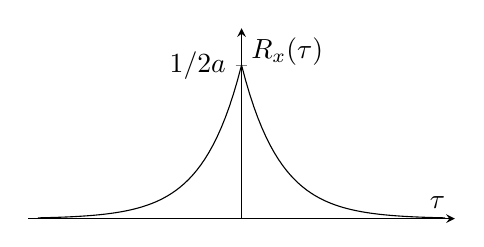
\begin{tikzpicture}
  \begin{axis}[width=7cm, height=4cm, axis lines=middle, xlabel={$\tau$}, ylabel={$R_x(\tau)$},
      xmin=-2.2, xmax=2.2, ymin=0, ymax=0.62, xtick=\empty, ytick={0.5}, yticklabels={$1/2a$}]
    \addplot[domain=-2.1:2.1, samples=101] {0.5*exp(-2.5*abs(x))};
  \end{axis}
\end{tikzpicture}
\end{center}
\[
  E_x=R_x(0)=\frac{1}{2a}
\]
\[
  R_x(\tau)=\frac{e^{-a|\tau|}}{2a}\ \xleftrightarrow{\ \mathcal{F}\ }\ \mathcal{E}_x(f)=\frac{1}{a^2+(2\pi f)^2}
\]
\formulkutu{e^{-a|\tau|},\ \tau>0\ \xleftrightarrow{\ \mathcal{F}\ }\ \frac{2a}{a^2+(2\pi f)^2}\footnotemark}
\footnotetext{Claude notu: koşul muhtemelen $a>0$ olmalı.}

\section{Güç ve Güç yoğunluk fonk (GYF)}
\sayfa{6}
\subsection{Power Spectral Density (PSD)}
\elcizimi[0.6]{sekiller/Ders5-s6-1.png}[6]
\[
  x_T(t)=\begin{cases} x(t), & |t|\le \dfrac{T}{2} \\[2mm] 0, & |t|>\dfrac{T}{2} \end{cases}
\]
\[
  x(t)\ \text{reel}\ \Rightarrow\ P_x=\lim_{T\to\infty}\frac{1}{T}\underbrace{\int_{-T/2}^{T/2}x^2(t)\,dt}_{E_{x_T}}=\lim_{T\to\infty}\frac{E_{x_T}}{T}
\]
\begin{align*}
  & x_T(t)\ \xleftrightarrow{\ \mathcal{F}\ }\ X_T(f) \\
  & E_{x_T}=\int_{-\infty}^{\infty}x_T^2(t)\,dt=\int_{-\infty}^{\infty}|X_T(f)|^2\,df
\end{align*}
\[
  P_x=\lim_{T\to\infty}\frac{E_{x_T}}{T}=\lim_{T\to\infty}\frac{1}{T}\Big[\int_{-\infty}^{\infty}|X_T(f)|^2\,df
\]
\[
  T\nearrow\ \Rightarrow\ x_T(t)\text{'nin süresi}\ \nearrow\ \Rightarrow\ E_{x_T}\nearrow\ \Rightarrow\ |X_T(f)|^2\nearrow
\]
\[
  P_x=\int_{-\infty}^{+\infty}\underbrace{\lim_{T\to\infty}\frac{1}{T}|X_T(f)|^2}_{\substack{=S_x(f)\\ \text{Güç yoğunluk fonk}}}\,df=\int_{-\infty}^{+\infty}S_x(f)\,df
\]
EYF, GYF pozitif, reel, çift f.

$x(t)$ birimi volt $\rightarrow$ volt$^2$/Hz

\section{Güç işaretlerinin özilişki fonk}
\sayfa{7}
$x(t)$ güç işareti $\Rightarrow$
\begin{align*}
  R_x(\tau) &= \lim_{T\to\infty}\frac{1}{T}\int_{-T/2}^{T/2}x(t)\cdot x^*(t-\tau)\,dt \\
  R_x(-\tau) &= R_x(\tau)
\end{align*}
\[
  R_x(\tau)\ \xleftrightarrow{\ \mathcal{F}\ }\ S_x(f)=\lim_{T\to\infty}\frac{|X_T(f)|^2}{T}
\]
\[
  R_x(0)=\lim_{T\to\infty}\frac{1}{T}\int_{-T/2}^{T/2}|x(t)|^2\,dt=P_x
\]
\[
  P_x=\lim_{T\to\infty}\frac{1}{T}\int_{-T/2}^{T/2}|x(t)|^2\,dt=R_x(0)=\int_{-\infty}^{\infty}S_x(f)\,df
\]
\begin{center}
\begin{tikzpicture}[>=Stealth, line width=0.7pt]
  \node[draw, minimum width=2cm, minimum height=1cm] (h) at (0,0) {$h(t)$};
  \draw[->] (-2.8,0) -- (h.west);
  \node[below] at (-2.2,0) {$x(t)$};
  \draw[->] (h.east) -- (2.8,0);
  \node[below] at (2.3,0) {$y(t)$};
\end{tikzpicture}
\end{center}
güç işareti:
\[
  y(t)=x(t)\ast h(t)=\int_{-\infty}^{\infty}x(\tau)\,h(t-\tau)\,d\tau
\]
güç işareti: \quad $R_y(\tau)=\displaystyle\lim_{T\to\infty}\frac{1}{T}\int_{-T/2}^{T/2}y(t)\,y^*(t-\tau)\,dt$

\elcizimi[0.3]{sekiller/Ders5-s7-1.png}[7]
\formulkutu{R_y(\tau)=R_x(\tau)\ast\underbrace{h(\tau)\ast h^*(-\tau)}_{R_h(\tau)}}
\[
  \downarrow\mathcal{F}
\]
\[
  S_y(f)=S_x(f)\cdot H(f)\cdot H^*(f)
\]
\formulkutu{S_y(f)=S_x(f)\,|H(f)|^2}

\begin{ornek}
  \begin{center}
  \begin{tikzpicture}[>=Stealth, line width=0.7pt]
    \node[draw, minimum width=1.6cm, minimum height=1.4cm] (d) at (0,0) {$\dfrac{d}{dt}$};
    \draw[->] (-2.6,0) -- (d.west);
    \node[below] at (-2.0,0) {$n_i(t)$};
    \draw[->] (d.east) -- (2.6,0);
    \node[below] at (2.0,0) {$n_o(t)$};
    \node at (5.6,0) {$H(f)=j2\pi f$};
  \end{tikzpicture}

  \medskip
  \begin{tikzpicture}[>=Stealth, line width=0.7pt]
    \draw[->] (-3,0) -- (3,0);
    \draw[->] (0,0) -- (0,1.9) node[above] {$S_{n_i}(f)$};
    \draw (-1.2,0) -- (-1.2,1.1) -- (1.2,1.1) -- (1.2,0);
    \node[above right] at (0,1.1) {$k$};
    \node[below] at (-1.2,0) {$-B$};
    \node[below] at (1.2,0) {$B$};
  \end{tikzpicture}
  \end{center}
  $n_i(t)$ is noise signal with PSD
  \[
    S_{n_i}(f)=\begin{cases} k, & |f|\le B \\ 0, & \text{else} \end{cases}
  \]
  $S_{n_o}(f)=\,$? \qquad $P_{n_o}=\,$?
\end{ornek}

\sayfa{8}
\begin{align*}
  S_{n_o}(f) &= S_{n_i}(f)\,|H(f)|^2 \\
  &= \begin{cases} k\cdot 4\pi^2 f^2, & |f|\le B \\ 0, & \text{Else} \end{cases}
\end{align*}
\begin{center}
\begin{tikzpicture}[>=Stealth, line width=0.7pt]
  \draw[->] (-2.6,0) -- (2.6,0) node[right] {$f$};
  \draw[->] (0,0) -- (0,2.4);
  \node[right] at (0,2.2) {$S_{n_o}(f)$};
  \node[right] at (0,1.85) {$k4\pi^2B^2$};
  \draw (-1.2,0) -- (-1.2,1.6);
  \draw (1.2,0) -- (1.2,1.6);
  \draw[domain=-1.2:1.2, samples=50, smooth] plot (\x,{1.6*(\x/1.2)^2});
  \draw[dashed] (-1.2,1.6) -- (1.2,1.6);
  \node[below] at (-1.2,0) {$-B$};
  \node[below] at (1.2,0) {$B$};
\end{tikzpicture}
\end{center}
\[
  P_{n_o}=\int_{-\infty}^{\infty}S_{n_o}(f)\,df=\int_{-B}^{B}k\,4\pi^2B^2f^2\,df\footnotemark
\]
\footnotetext{Claude notu: integrandda $B^2$ çarpanı muhtemelen fazla ($S_{n_o}(f)=k\cdot4\pi^2f^2$); sonuç $8k\pi^2B^3/3$ ile uyumlu olması için integrand $k\,4\pi^2f^2$ olmalı.}
\[
  =\frac{8k\pi^2B^3}{3}
\]

\begin{ornek}
  $x(t)$ periyodik $\Rightarrow\ R_x(\tau)=\,$? \quad $S_x(f)=\,$?
\end{ornek}
$\Downarrow$ (güç)
\[
  R_x(\tau)=\frac{1}{T_0}\int_{-T_0/2}^{T_0/2}x(t)\cdot x^*(t-\tau)\,dt
\]
$x(t)$ periyodik $\Rightarrow\ x(t)=\displaystyle\sum_{n=-\infty}^{\infty}x_n\,e^{j2\pi n f_0 t}$
\begin{align*}
  R_x(\tau) &= \frac{1}{T_0}\int_{-T_0/2}^{T_0/2}\underbrace{\sum_{n=-\infty}^{\infty}x_n\,e^{j2\pi n f_0 t}}_{x(t)}
  \cdot\underbrace{\sum_{m=-\infty}^{+\infty}x_m^*\,e^{-j2\pi m f_0(t-\tau)}}_{x^*(t)}\,dt \\
  &= \frac{1}{T_0}\sum_{n=-\infty}^{+\infty}\sum_{m=-\infty}^{\infty}x_n\,x_m^*\,e^{j2\pi m f_0\tau} \\
  &\qquad\underbrace{\int_{-T_0/2}^{T_0/2}e^{j2\pi n f_0 t}\cdot e^{-j2\pi m f_0 t}\,dt}_{\begin{cases} T_0, & n=m \\ 0, & n\neq m \end{cases}}
\end{align*}
\[
  \kutula{R_x(\tau)=\sum_{n=-\infty}^{+\infty}|x_n|^2\,e^{j2\pi n f_0\tau}}
  \ \longleftrightarrow\ S_x(f)=\sum_{n=-\infty}^{+\infty}|x_n^2|\,\delta(f-nf_0)
\]
Periyodik işaretin öz fonksiyonu periyodiktir
\begin{align*}
  \rightarrow\ P_x &= \int_{-\infty}^{+\infty}S_x(f)\,df=\int_{-\infty}^{\infty}\sum_{n=-\infty}^{\infty}|x_n|^2\,\delta(f-nf_0)\,df \\
  &= \sum_n|x_n|^2\underbrace{\int_{-\infty}^{+\infty}\delta(f-nf_0)\,df}_{1} \qquad P_x=\sum_{n=-\infty}^{\infty}|x_n|^2
\end{align*}
\end{document}
